\documentclass{beamer}
\usepackage{graphicx} % Required for inserting images
\usepackage{hyperref}

\title{Instalacion R}
\author{Miguel Beltrá Vidal}
\date{Septiembre 2026}

\begin{document}

\maketitle

\section{Instalación de R}

\begin{frame}{}
    \begin{center}
        \Huge \secname
    \end{center}
\end{frame}


\begin{frame}{}
    \begin{center}
        \url{https://www.r-project.org/}
    \end{center}

    \begin{figure}
        \centering
        
\includegraphics[width=0.9\linewidth]{images/instalacion_R_1.png}
    \end{figure}
\end{frame}


\begin{frame}{}
    \begin{figure}
        \centering
        
\includegraphics[width=\linewidth]{images/instalacion_R_2.png}
    \end{figure}
\end{frame}


\begin{frame}{}
    \begin{figure}
        \centering
        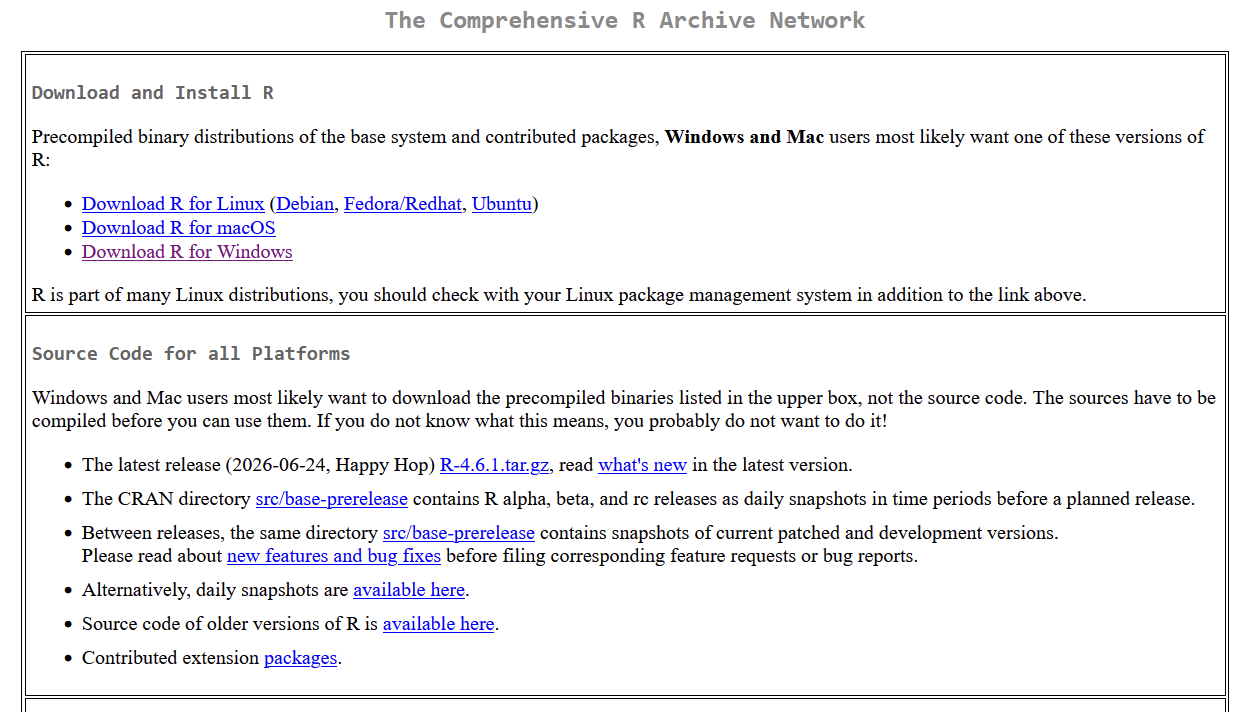
\includegraphics[width=\linewidth]{images/instalacion_R_3.png}
    \end{figure}
\end{frame}


\begin{frame}{}
    \begin{figure}
        \centering
        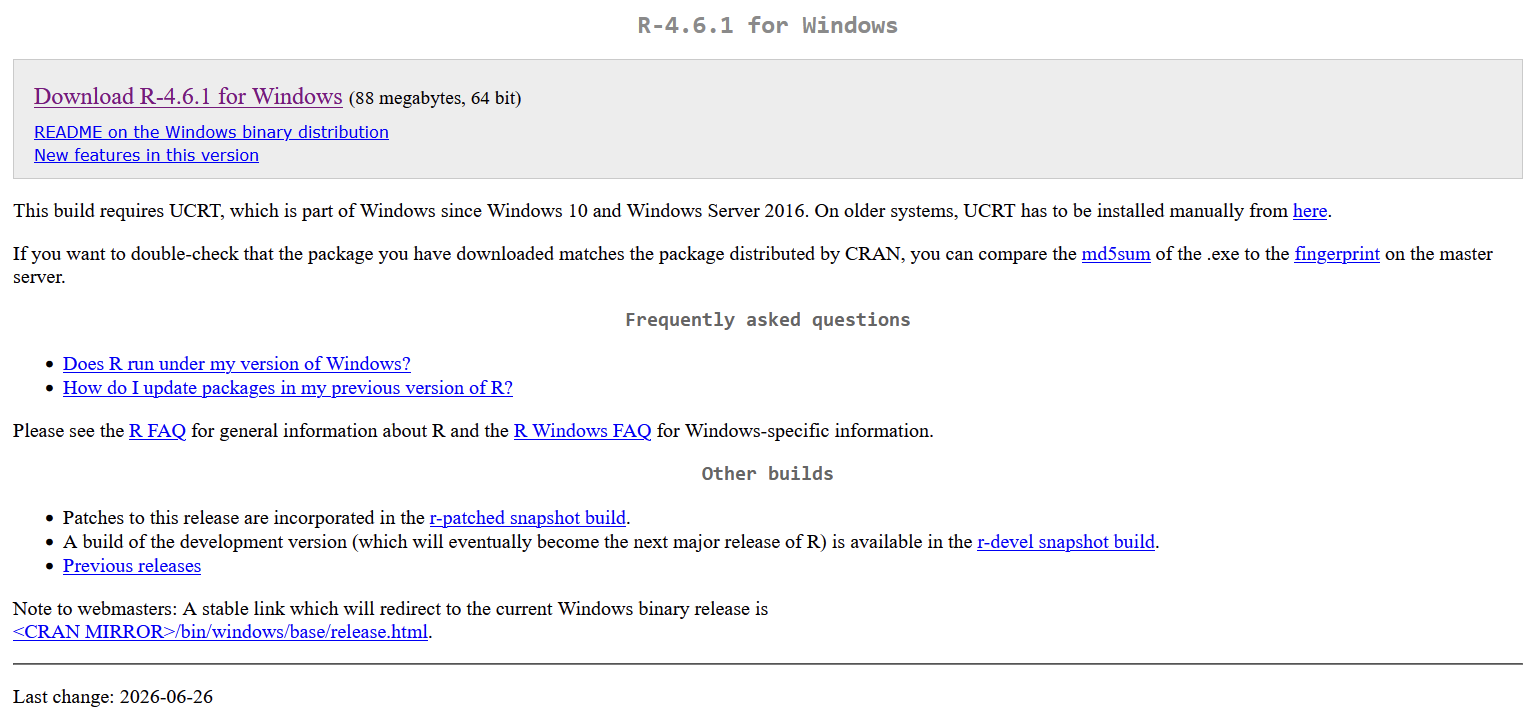
\includegraphics[width=\linewidth]{images/instalacion_R_4.png}
    \end{figure}
\end{frame}


\begin{frame}{}
    \begin{figure}
        \centering
        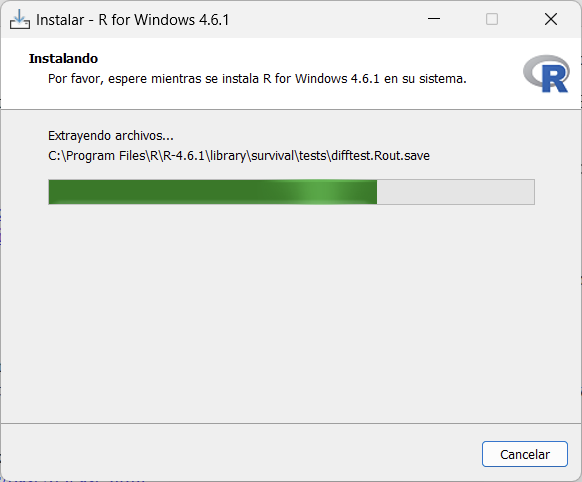
\includegraphics[width=\linewidth]{images/instalacion_R_5.png}
    \end{figure}
\end{frame}


\section{Instalación de RStudio}

\begin{frame}{}
    \begin{center}
        \Huge \secname
    \end{center}
\end{frame}


\begin{frame}{}
    \begin{figure}
        \centering
        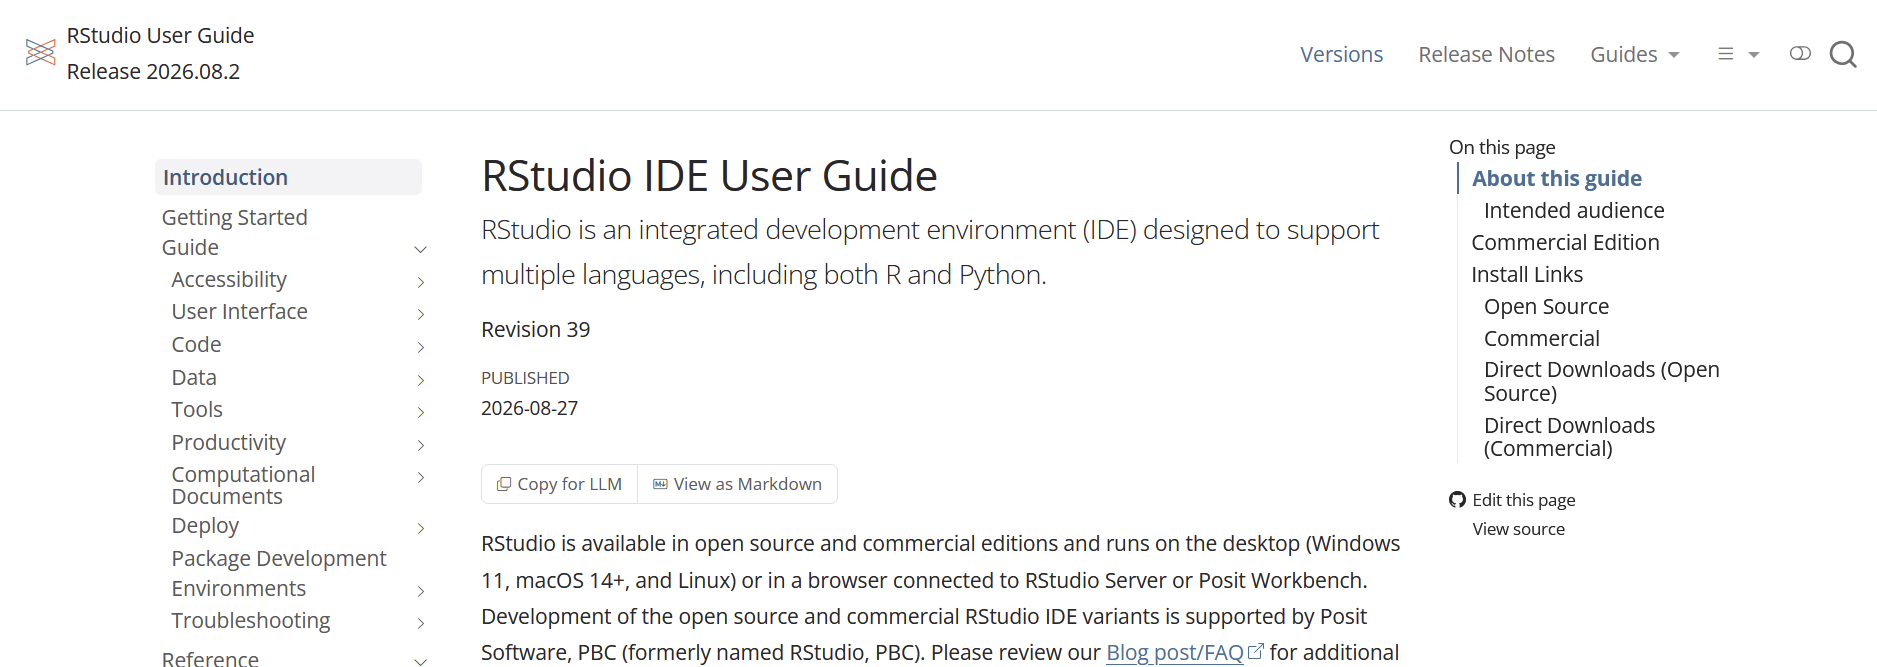
\includegraphics[width=\linewidth]{images/instalacion_RStudio_1.png}
    \end{figure}
\end{frame}


\begin{frame}{}
    \begin{figure}
        \centering
        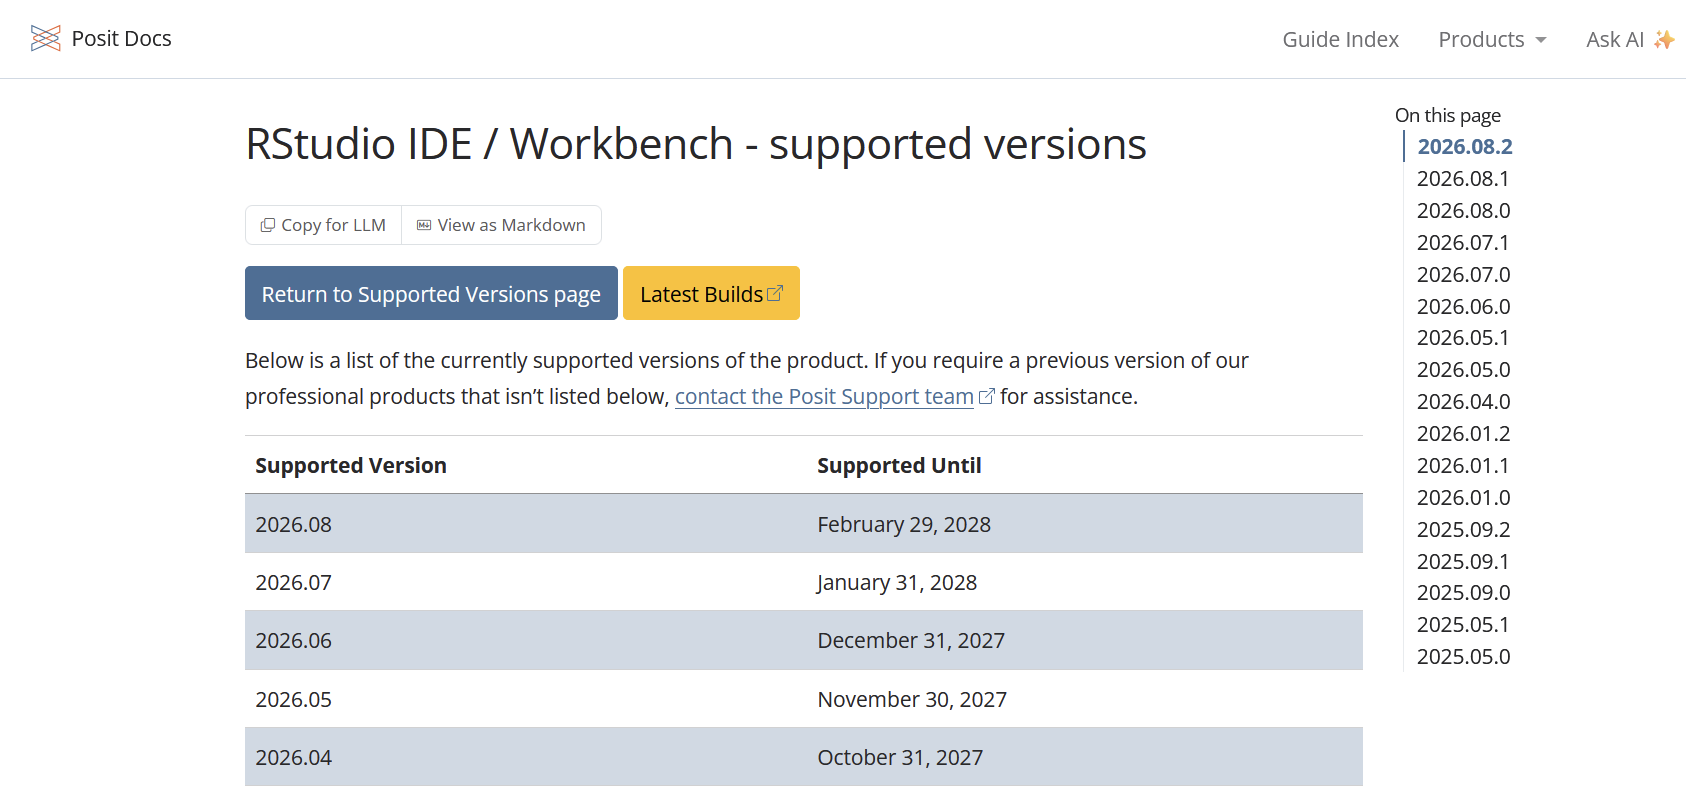
\includegraphics[width=1\linewidth]{images/instalacion_RStudio_2.png}
    \end{figure}
\end{frame}


\begin{frame}{}

    En esa página, un poco más abajo, se encuentran los enlaces a los instaladores de las distintas versiones:

    \begin{figure}
        \centering
        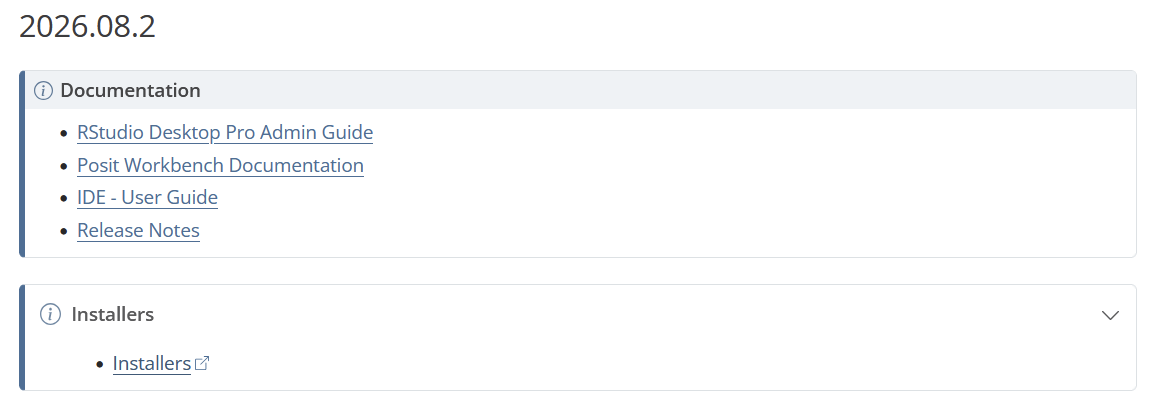
\includegraphics[width=1\linewidth]{images/instalacion_RStudio_3.png}
    \end{figure}
\end{frame}


\begin{frame}{}
    \begin{figure}
        \centering
        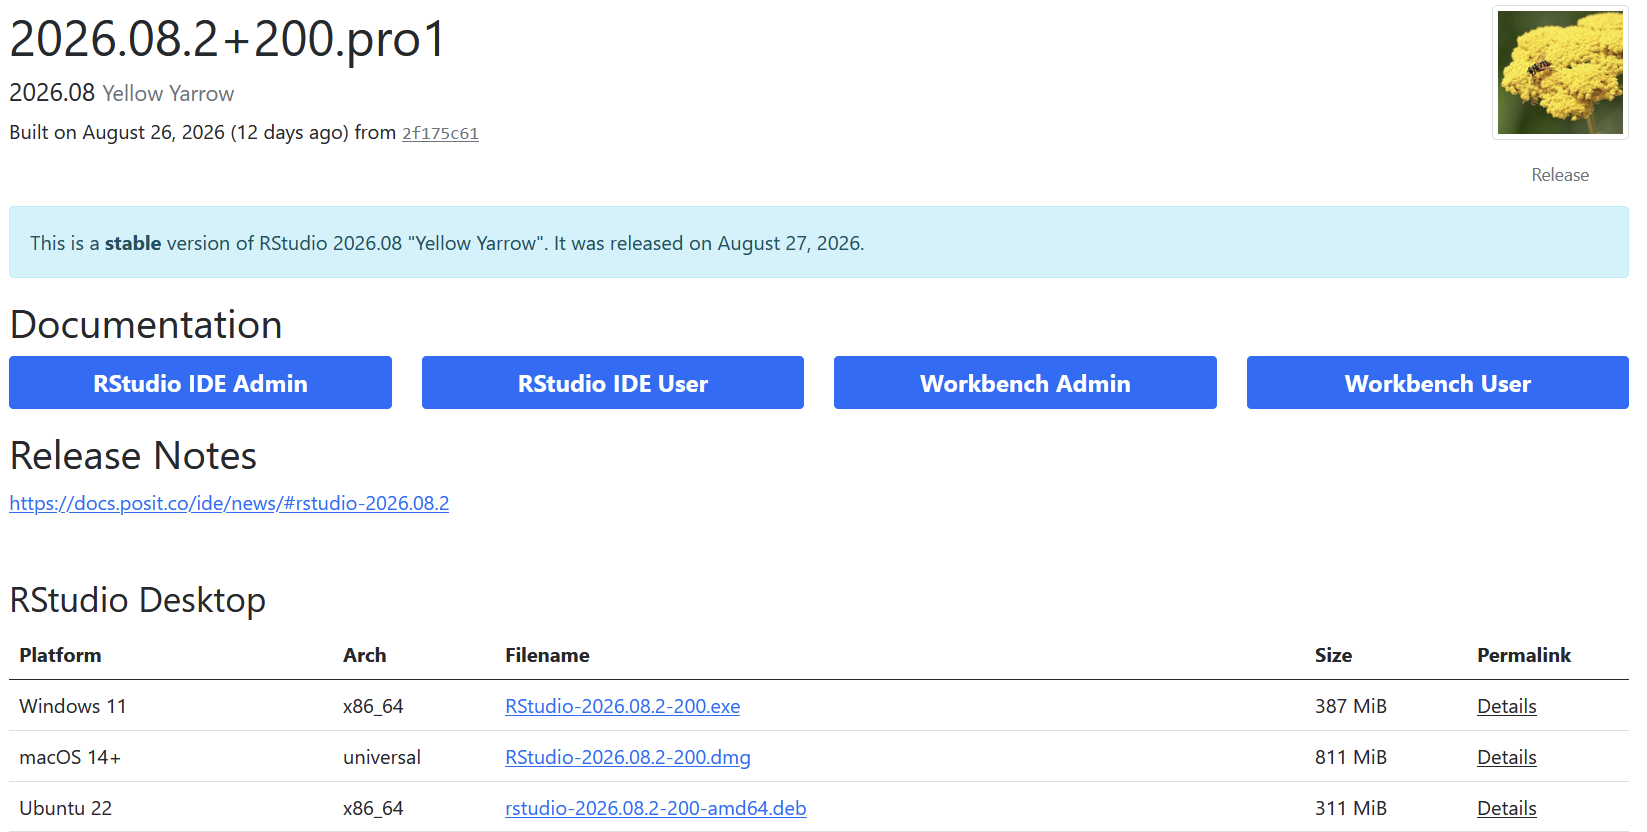
\includegraphics[width=1\linewidth]{images/instalacion_RStudio_4.png}
    \end{figure}
\end{frame}


\begin{frame}{}

    Ejecutamos el instalador descargado:

    \begin{figure}
        \centering
        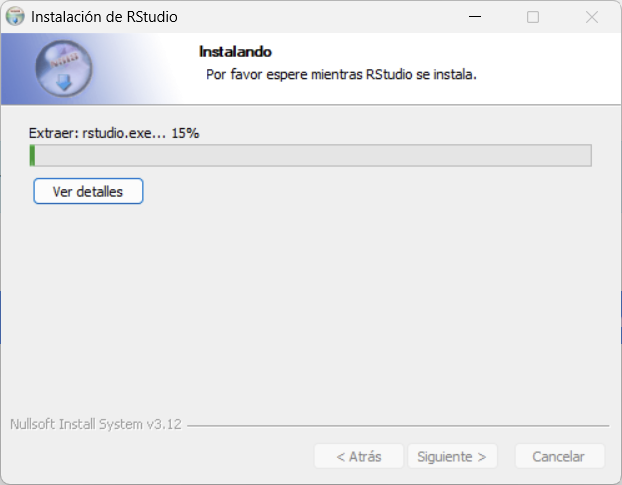
\includegraphics[width=0.75\linewidth]{images/instalacion_RStudio_5.png}
    \end{figure}
\end{frame}


\section{Configuración de RStudio}

\begin{frame}{}
    \begin{center}
        \Huge \secname
    \end{center}
\end{frame}


\begin{frame}{}
    \begin{figure}
        \centering
        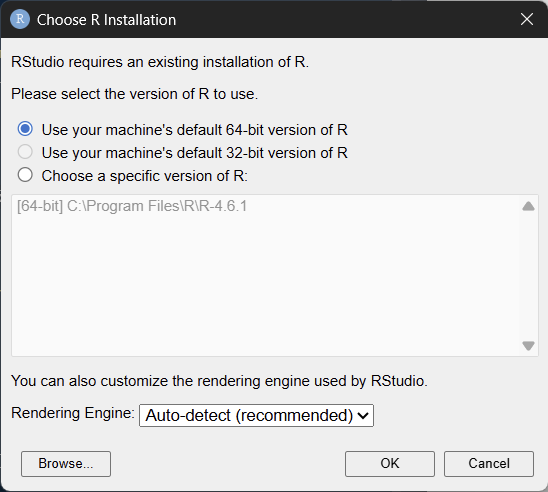
\includegraphics[width=0.75\linewidth]{images/configuracion_1.png}
    \end{figure}    
\end{frame}


\begin{frame}{}
    \begin{figure}
        \centering
        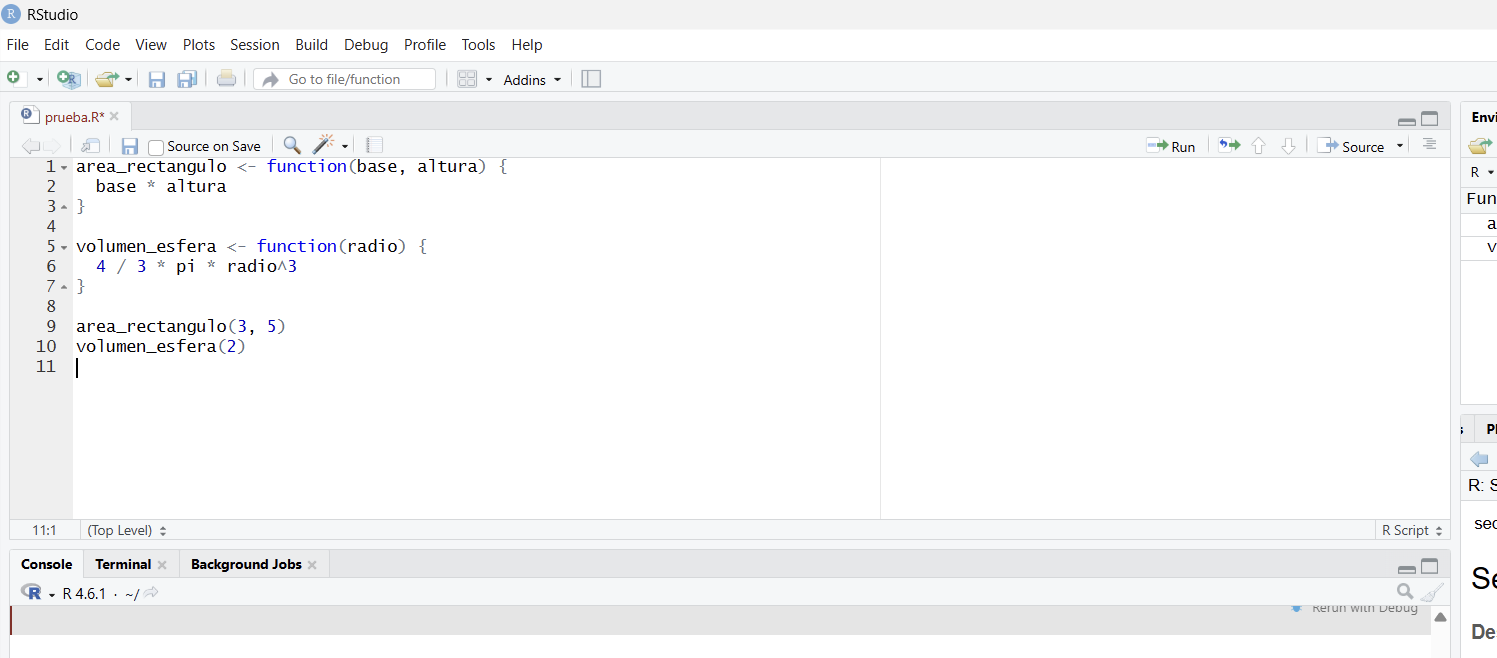
\includegraphics[width=1\linewidth]{images/funcion_1.png}
    \end{figure}    
\end{frame}


\begin{frame}{}
    Podemos ejecutar el código con el boton \texttt{Run}
    \begin{figure}
        \centering
        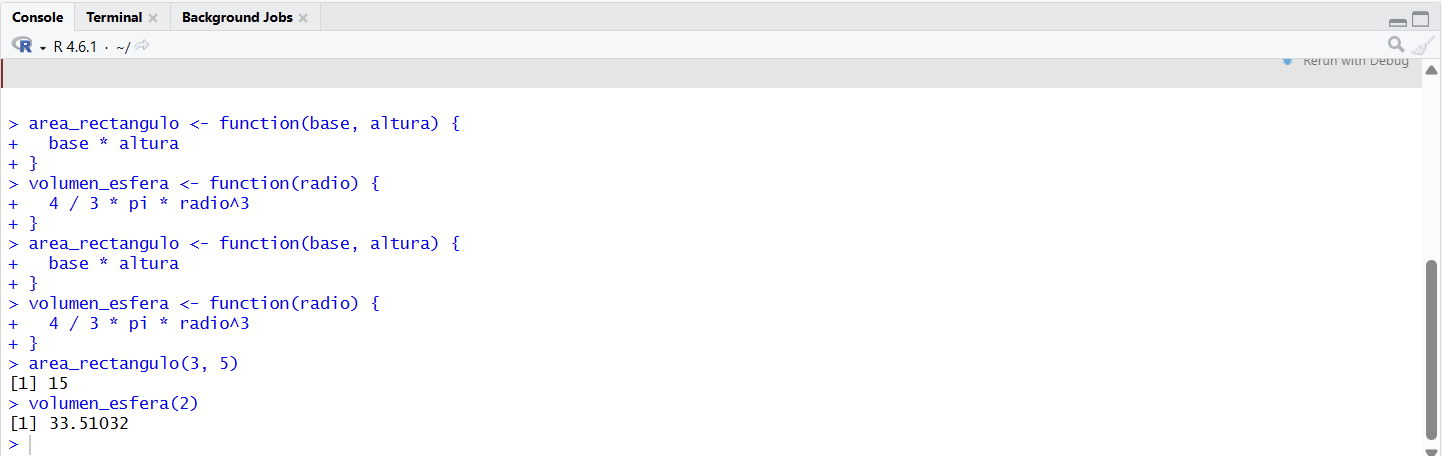
\includegraphics[width=1\linewidth]{images/funcion_2.png}
    \end{figure}
\end{frame}


\end{document}
